\documentclass[]{book}
\usepackage{lmodern}
\usepackage{amssymb,amsmath}
\usepackage{ifxetex,ifluatex}
\usepackage{fixltx2e} % provides \textsubscript
\ifnum 0\ifxetex 1\fi\ifluatex 1\fi=0 % if pdftex
  \usepackage[T1]{fontenc}
  \usepackage[utf8]{inputenc}
\else % if luatex or xelatex
  \ifxetex
    \usepackage{mathspec}
  \else
    \usepackage{fontspec}
  \fi
  \defaultfontfeatures{Ligatures=TeX,Scale=MatchLowercase}
\fi
% use upquote if available, for straight quotes in verbatim environments
\IfFileExists{upquote.sty}{\usepackage{upquote}}{}
% use microtype if available
\IfFileExists{microtype.sty}{%
\usepackage{microtype}
\UseMicrotypeSet[protrusion]{basicmath} % disable protrusion for tt fonts
}{}
\usepackage[margin=1in]{geometry}
\usepackage{hyperref}
\hypersetup{unicode=true,
            pdftitle={R Freamworkleri},
            pdfauthor={Metin YALÇINKAYA},
            pdfborder={0 0 0},
            breaklinks=true}
\urlstyle{same}  % don't use monospace font for urls
\usepackage{natbib}
\bibliographystyle{apalike}
\usepackage{color}
\usepackage{fancyvrb}
\newcommand{\VerbBar}{|}
\newcommand{\VERB}{\Verb[commandchars=\\\{\}]}
\DefineVerbatimEnvironment{Highlighting}{Verbatim}{commandchars=\\\{\}}
% Add ',fontsize=\small' for more characters per line
\usepackage{framed}
\definecolor{shadecolor}{RGB}{248,248,248}
\newenvironment{Shaded}{\begin{snugshade}}{\end{snugshade}}
\newcommand{\KeywordTok}[1]{\textcolor[rgb]{0.13,0.29,0.53}{\textbf{#1}}}
\newcommand{\DataTypeTok}[1]{\textcolor[rgb]{0.13,0.29,0.53}{#1}}
\newcommand{\DecValTok}[1]{\textcolor[rgb]{0.00,0.00,0.81}{#1}}
\newcommand{\BaseNTok}[1]{\textcolor[rgb]{0.00,0.00,0.81}{#1}}
\newcommand{\FloatTok}[1]{\textcolor[rgb]{0.00,0.00,0.81}{#1}}
\newcommand{\ConstantTok}[1]{\textcolor[rgb]{0.00,0.00,0.00}{#1}}
\newcommand{\CharTok}[1]{\textcolor[rgb]{0.31,0.60,0.02}{#1}}
\newcommand{\SpecialCharTok}[1]{\textcolor[rgb]{0.00,0.00,0.00}{#1}}
\newcommand{\StringTok}[1]{\textcolor[rgb]{0.31,0.60,0.02}{#1}}
\newcommand{\VerbatimStringTok}[1]{\textcolor[rgb]{0.31,0.60,0.02}{#1}}
\newcommand{\SpecialStringTok}[1]{\textcolor[rgb]{0.31,0.60,0.02}{#1}}
\newcommand{\ImportTok}[1]{#1}
\newcommand{\CommentTok}[1]{\textcolor[rgb]{0.56,0.35,0.01}{\textit{#1}}}
\newcommand{\DocumentationTok}[1]{\textcolor[rgb]{0.56,0.35,0.01}{\textbf{\textit{#1}}}}
\newcommand{\AnnotationTok}[1]{\textcolor[rgb]{0.56,0.35,0.01}{\textbf{\textit{#1}}}}
\newcommand{\CommentVarTok}[1]{\textcolor[rgb]{0.56,0.35,0.01}{\textbf{\textit{#1}}}}
\newcommand{\OtherTok}[1]{\textcolor[rgb]{0.56,0.35,0.01}{#1}}
\newcommand{\FunctionTok}[1]{\textcolor[rgb]{0.00,0.00,0.00}{#1}}
\newcommand{\VariableTok}[1]{\textcolor[rgb]{0.00,0.00,0.00}{#1}}
\newcommand{\ControlFlowTok}[1]{\textcolor[rgb]{0.13,0.29,0.53}{\textbf{#1}}}
\newcommand{\OperatorTok}[1]{\textcolor[rgb]{0.81,0.36,0.00}{\textbf{#1}}}
\newcommand{\BuiltInTok}[1]{#1}
\newcommand{\ExtensionTok}[1]{#1}
\newcommand{\PreprocessorTok}[1]{\textcolor[rgb]{0.56,0.35,0.01}{\textit{#1}}}
\newcommand{\AttributeTok}[1]{\textcolor[rgb]{0.77,0.63,0.00}{#1}}
\newcommand{\RegionMarkerTok}[1]{#1}
\newcommand{\InformationTok}[1]{\textcolor[rgb]{0.56,0.35,0.01}{\textbf{\textit{#1}}}}
\newcommand{\WarningTok}[1]{\textcolor[rgb]{0.56,0.35,0.01}{\textbf{\textit{#1}}}}
\newcommand{\AlertTok}[1]{\textcolor[rgb]{0.94,0.16,0.16}{#1}}
\newcommand{\ErrorTok}[1]{\textcolor[rgb]{0.64,0.00,0.00}{\textbf{#1}}}
\newcommand{\NormalTok}[1]{#1}
\usepackage{longtable,booktabs}
\usepackage{graphicx,grffile}
\makeatletter
\def\maxwidth{\ifdim\Gin@nat@width>\linewidth\linewidth\else\Gin@nat@width\fi}
\def\maxheight{\ifdim\Gin@nat@height>\textheight\textheight\else\Gin@nat@height\fi}
\makeatother
% Scale images if necessary, so that they will not overflow the page
% margins by default, and it is still possible to overwrite the defaults
% using explicit options in \includegraphics[width, height, ...]{}
\setkeys{Gin}{width=\maxwidth,height=\maxheight,keepaspectratio}
\IfFileExists{parskip.sty}{%
\usepackage{parskip}
}{% else
\setlength{\parindent}{0pt}
\setlength{\parskip}{6pt plus 2pt minus 1pt}
}
\setlength{\emergencystretch}{3em}  % prevent overfull lines
\providecommand{\tightlist}{%
  \setlength{\itemsep}{0pt}\setlength{\parskip}{0pt}}
\setcounter{secnumdepth}{5}
% Redefines (sub)paragraphs to behave more like sections
\ifx\paragraph\undefined\else
\let\oldparagraph\paragraph
\renewcommand{\paragraph}[1]{\oldparagraph{#1}\mbox{}}
\fi
\ifx\subparagraph\undefined\else
\let\oldsubparagraph\subparagraph
\renewcommand{\subparagraph}[1]{\oldsubparagraph{#1}\mbox{}}
\fi

%%% Use protect on footnotes to avoid problems with footnotes in titles
\let\rmarkdownfootnote\footnote%
\def\footnote{\protect\rmarkdownfootnote}

%%% Change title format to be more compact
\usepackage{titling}

% Create subtitle command for use in maketitle
\newcommand{\subtitle}[1]{
  \posttitle{
    \begin{center}\large#1\end{center}
    }
}

\setlength{\droptitle}{-2em}
  \title{R Freamworkleri}
  \pretitle{\vspace{\droptitle}\centering\huge}
  \posttitle{\par}
  \author{Metin YALÇINKAYA}
  \preauthor{\centering\large\emph}
  \postauthor{\par}
  \predate{\centering\large\emph}
  \postdate{\par}
  \date{2018}

\usepackage{booktabs}
\usepackage{amsthm}
\makeatletter
\def\thm@space@setup{%
  \thm@preskip=8pt plus 2pt minus 4pt
  \thm@postskip=\thm@preskip
}
\makeatother

\begin{document}
\maketitle

{
\setcounter{tocdepth}{1}
\tableofcontents
}
\chapter{Giriş}\label{giris}

\begin{figure}
\centering

\includegraphics{resim0.png}
\caption{}
\end{figure}

\section{Tanıtım}\label{tantm}

Bu materyal R programlama dili ile ilgili freamworkler ile ilgili
yeterince Türkçe kaynak olmamasından ve bu konu ile ilgili olan
araştırmacılar için oluşturulmuştur. Bu materyalde freamworklerin
hakkında ayrıca nasıl oluşturacağınıza dair bir bazı bilgiler yer
almaktadır.

\section{Gereklilikler}\label{gereklilikler}

Bu materyalde yer alan uygulamları gerçekleştirebilmek için RStudio
kullanmış ve bir miktar programlama dersi görmüş olmanız yeterlidir.\\
Ayrıca bilgisayarınızda \href{https://www.r-project.org/}{R} ve
\href{https://www.rstudio.com/}{RStudio} kurulu olmalıdır.

\chapter{Bookdown}\label{intro}

Bookdown Rmarkdown üzerine kurulu bir kitap, makale oluşturmanızı
sağlayan bir R freamworküdür. Resmi sitesinde tanımlandığı şekilde;

``Bookdown, şekil / tablo başlık numaralandırma ve çapraz referanslar
gibi kitap yazma ile ilgili birkaç önemli eksik özelliği ekleyerek ve
HTML widget'larını veya Parlak uygulamaların gömülmesini içerir. Tüm
çıktı biçimleri için (PDF, HTML ve EPUB, vb.) Her şeyi yapmaya çalıştık,
böylece okuyucularınız okumak için en sevdikleri dosya formatını
seçebilirler. Bookdown paketi R kullanılarak geliştirilmesine rağmen,
kitabınızın R ile ilgili olması gerektiği anlamına gelmez. Kesinlikle
şiirleri veya romanları yazabilirsin!''

gibi bir açıklamaları bulunur.

\section{Gereklilikler}\label{gereklilikler-1}

RStudio'yu açıp konsol kısmına aşağıdaki komutu yapıştırarak gerekli
paketlerin kurulmasını sağlayabilirsiniz;

\begin{Shaded}
\begin{Highlighting}[]
\KeywordTok{install.packages}\NormalTok{(}\StringTok{"devtools"}\NormalTok{)}
\NormalTok{  devtools}\OperatorTok{::}\KeywordTok{install_github}\NormalTok{(}\StringTok{"rstudio/bookdown"}\NormalTok{)}
\end{Highlighting}
\end{Shaded}

\begin{Shaded}
\begin{Highlighting}[]
\KeywordTok{install.packages}\NormalTok{(}\StringTok{"bookdown"}\NormalTok{)}
\end{Highlighting}
\end{Shaded}

paketler ile işimiz bittiğine göre şimdide bir template dosyası
indirmemiz gerekiyor.
\href{https://github.com/rstudio/bookdown-demo}{Buradan} template
dosyasını indiriniz.

\section{Başlangıç}\label{baslangc}

İlk olarak indirdiğimiz .zip dosyasını çıkartıyoruz. Bu dosya içerisinde
bir template olarak hazırlanmış örnek bir kitap yer almaktadır.

\textbf{index.Rmd}\\
Bu dosya materyalinizin kapak kısmı denilebilir. Bu kısım içerisinde
kitap hakkında bilgi, yazar, yıl gibi bilgiler yer alabilir. Aşağıdaki
resimlerin ilkinde index.Rmd dosyasının RStudio ile kodlandığı alan
gösterilmektedir.

\begin{figure}
\centering
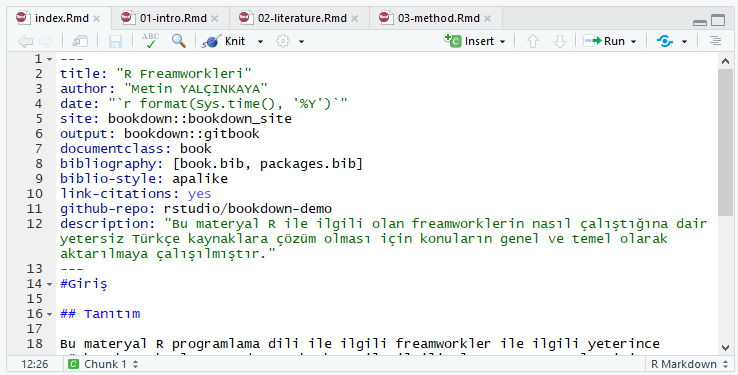
\includegraphics{resim1.png}
\caption{}
\end{figure}

Burada ise Rstudio içerisindeki düzenlemelerden sonra kitabın önizlemesi
gösterilmektedir.

\begin{figure}
\centering
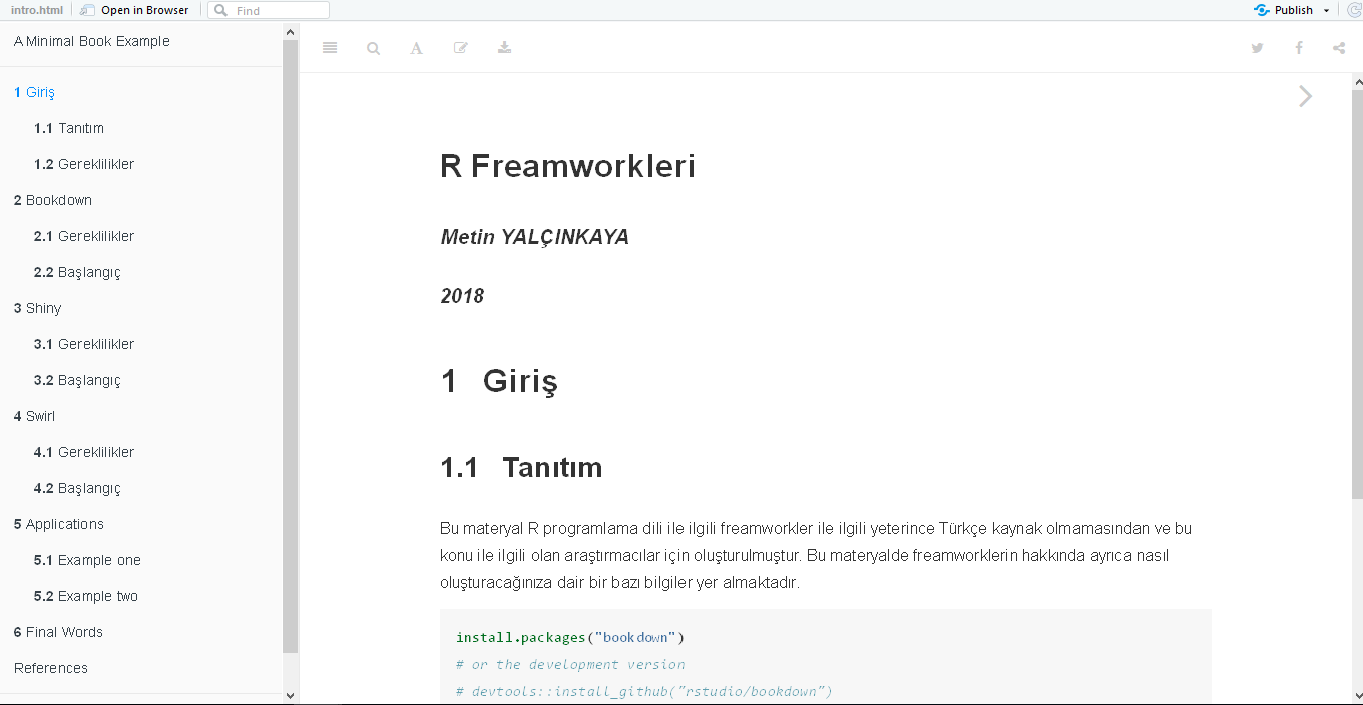
\includegraphics{resim2.png}
\caption{}
\end{figure}

\textbf{intro.Rmd}\\
Bu bölüm adındanda anlaşılacağı üzere giriş kısmıdır. Bu bölüm
içerisinde öğrenene temel bilgiler verilmektedir.

\section{Düzenleme}\label{duzenleme}

Yukarıdaki temel bilgileri aldığınıza göre sıra şimdi dosyaları
düzenleme aşamasına geldi. Dosyalar Rmarkdown ve markdown ile düzenleme
yapılarak sayfaları oluşturulur. Rmarkdown ile markdown arasında birkaç
farklılık dışında başka birşey yoktur. Aşağıda ise kitabınıza
yapabileceğiniz düzenlemelerin nasıl olduğu gösterilmektedir.

\subsection{Başlık}\label{baslk}

Materyaliniz içerisindeki başlıklandırma işlemlerini yapmanız için
kullanılır. ``\#'' simgesi kullanılarak yapılır ve aynı h1\ldots{}h6
gibi \# sayısı arttırılarak başlık belirlenir.

\begin{Shaded}
\begin{Highlighting}[]
\NormalTok{##Başlık1}
\NormalTok{###Başlık2}
\NormalTok{####Başlık3}
\end{Highlighting}
\end{Shaded}

\subsection{Link}\label{link}

Metniniz içerisinde kelimeye bir url eklemeniz gerektiği durumlarda
kullanabilirsiniz. Köşeli parantezler içerisine metin girilir, hemen
yanına boşluk bırakılmadan parantez açılır ve url adresi girilir.

\begin{Shaded}
\begin{Highlighting}[]
\OtherTok{[Link Verilecek Metin](URL Adresi)}
\end{Highlighting}
\end{Shaded}

\subsection{Liste}\label{liste}

Adındanda anlaşılacağı üzere bir nesne grubunu listelemeniz gereken
durumlarda kullanabilirsiniz. Listeyi oluşturmak için ``+'' işareti veya
sayısal olarak listelemeniz gerekiyorsa ``1.'' den başlayarak arttırarak
listenizi oluşturabilirsiniz.

\begin{Shaded}
\begin{Highlighting}[]
\NormalTok{+ilk madde}
\NormalTok{+ikinci madde}
\end{Highlighting}
\end{Shaded}

\subsection{Kod Ekleme \& Renklendirme}\label{kod-ekleme-renklendirme}

Bu alan html içerisinde en zor olan alanlardan birisi bir metin
içerisinde bir sürü span ile farklı farklı cssler vererek düzenleme
yapılıyor fakat markdown sadece üç nokta içerisine hangi kodu
yazacağınızı belirtip yazabiliyorsunuz;

\begin{figure}
\centering
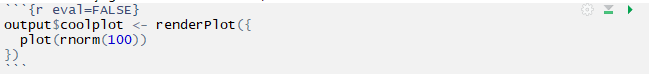
\includegraphics{resim9.png}
\caption{}
\end{figure}

\subsection{Tablo}\label{tablo}

Tablolama yapmanız gereken durumlarda aşağıdaki kod bloğunu
kullanabilirsiniz;

\begin{Shaded}
\begin{Highlighting}[]
\NormalTok{| Tables        | Are           | Cool  |}
\NormalTok{| ------------- |:-------------:| -----:|}
\NormalTok{| col 3 is      | right-aligned | $1600 |}
\NormalTok{| col 2 is      | centered      |   $12 |}
\NormalTok{| zebra stripes | are neat      |    $1 |}
\end{Highlighting}
\end{Shaded}

Tirelerin kullanıldığı blok bir üst bloğun başlıklar olduğunu
belirtiyor. Çıkıtısı da aşağıdaki gibi olacaktır;

\begin{longtable}[]{@{}lcr@{}}
\toprule
Tables & Are & Cool\tabularnewline
\midrule
\endhead
col 3 is & right-aligned & \$1600\tabularnewline
col 2 is & centered & \$12\tabularnewline
zebra stripes & are neat & \$1\tabularnewline
\bottomrule
\end{longtable}

\subsection{Resim}\label{resim}

Yazınız içerisinde eklemeniz gereken resimleri aşağıdaki kod bloğu ile
ekleyebiliriz.

\begin{Shaded}
\begin{Highlighting}[]
\NormalTok{![](resimadi.png)}
\end{Highlighting}
\end{Shaded}

\subsection{Daha Fazlası}\label{daha-fazlas}

Daha fazla içerik eklemek için Rmarkdown ingilizce kaynağı olan
\href{https://rmarkdown.rstudio.com/authoring_pandoc_markdown.html\#pandoc_markdown}{bu
adresi} ziyaret edebilirsiniz.

\section{Önizleme ve Çıktı Alma}\label{onizleme-ve-ckt-alma}

Materyaliniz üzerinde yeterince düzenleme yaptınız ve artık bir çıktı
önizleme yapmanız gerekiyor.\\
Öncelikle varsayalım tek bir sayfa üzerinde çıktı almak istiyorsanız
resimde gösterilen ``Knit'' butonuna tıklayın böylece sayfanızı
önizleyebilirsiniz; 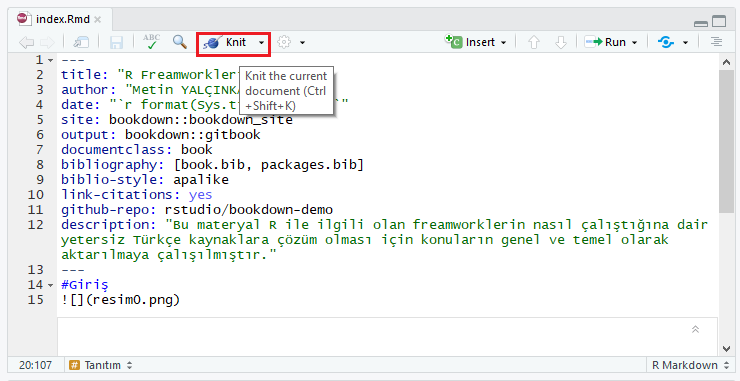
\includegraphics{resim3.png}

Bir problem yok şimdide bütün projenin ne durumda olduğunu görmek
istiyorsak ``Build'' menüsü altında ``Build All'' ile tüm projenin
hazırlanmasını sağlıyoruz ayrıca böylece sitenin html dosyalarının
hepsinin hazırlanmasını sağlıyoruz (bunlar \_book klasörü içerisinde yer
alır.) daha sonra bir önceki resimde olduğu gibi ``Knit'' butonuna
tıklayarak kitabın her menüsünü rahatlıkla inceleyebilir veya klasör
içerisindeki html dosyalarını bir tarayıcı üzerinden
görüntüleyebilirsiniz;

\begin{figure}
\centering
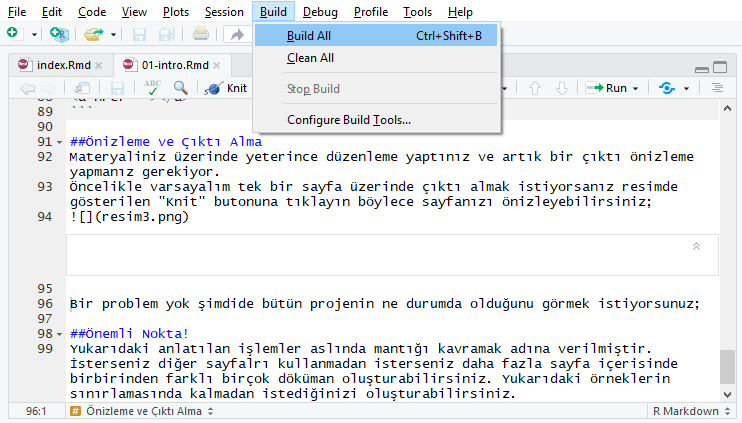
\includegraphics{resim4.png}
\caption{}
\end{figure}

\section{Önemli Nokta!}\label{onemli-nokta}

Yukarıdaki anlatılan işlemler aslında mantığı kavramak adına
verilmiştir. İsterseniz diğer sayfalrı kullanmadan isterseniz daha fazla
sayfa içerisinde birbirinden farklı birçok döküman oluşturabilirsiniz.
Yukarıdaki örneklerin sınırlamasında kalmadan istediğinizi
oluşturabilirsiniz.

\chapter{Shiny}\label{shiny}

Shiny etkileşimli web sayfalarını oluşturmanıza olanak sağlayan RStudio
paketidir. R kullanıcılarının yöneliktir ve html,css,js bilmenize gerek
yoktur.\\
Shiny ile oldukça fazla şey yapabilirsiniz: etkileşimli bir web sayfası
yapmanın kolay bir yolu olarak düşünün ve bu web sayfası R ile sorunsuz
bir şekilde etkileşime girebilir ve R nesnelerini (R'de yaptığınız her
şeyin grafikleri, tabloları) gösterebilir.

\section{Gereklilikler}\label{gereklilikler-2}

Shiny kullanabilmek için aşağıdaki paketi öncelikle yüklemelisiniz.

\begin{Shaded}
\begin{Highlighting}[]
\KeywordTok{install.packages}\NormalTok{(}\StringTok{"shiny"}\NormalTok{)}
\end{Highlighting}
\end{Shaded}

Ayrıca uygulama için kullanabileceğimiz veri setini
\href{https://deanattali.com/files/bcl-data.csv}{buradan} indirelim.

\section{Başlangıç}\label{baslangc-1}

Shiny uygulamaları iki bölümden oluşur. Bir bölümde kullanıcının
etkileşime girdiği web sayfası birde uygulamaya güç veren bir sunucu
tarafı olarak uygulamayı yazmanız gerekiyor. Kullanıcı arayüzü,
kullanıcının göreceği bir web dokümanıdır, Shiny'in işlevlerini
kullanarak yazdığınız HTML'dir. Kullanıcı Arayüzü, uygulamanın düzenini
oluşturup tüm şeylerin nereye gittiğini tam olarak söylemekle
sorumludur. Sunucu, uygulamanın mantığından sorumludur; Kullanıcı,
sayfayla etkileşimde bulunduğunda ne göstereceğini web sayfasına
bildiren talimatlar kümesidir.

Şimdi bir shiny uygulaması oluşturalım; ilk olarak shiny uygulamanızı
ister tek dosya halinde ister ui,server olarak iki dosya halinde
hazırlayabilirsiniz. Tek dosya halinde oluşturmak için RStudio üzerinde
oluşturduğunuz yeni dosya içerisine;

\begin{Shaded}
\begin{Highlighting}[]
\KeywordTok{library}\NormalTok{(shiny)}
\NormalTok{ui <-}\StringTok{ }\KeywordTok{fluidPage}\NormalTok{()}
\NormalTok{server <-}\StringTok{ }\ControlFlowTok{function}\NormalTok{(input, output) \{\}}
\KeywordTok{shinyApp}\NormalTok{(}\DataTypeTok{ui =}\NormalTok{ ui, }\DataTypeTok{server =}\NormalTok{ server)}
\end{Highlighting}
\end{Shaded}

kodları girerek shiny uygulamızın temel kodlarınız yazıyoruz.\emph{Bu
noktada önemli olan eğer uygulama tek dosyada yer alacaksa adı
\textbf{app.R} olmalıdır.} Bu işlemleri yaptık şimdi sıra kodu test etme
aşaması var. Bunun için Rstudio üzerindeki \textbf{Run App} butonuna
tıklayarak uygulamanızın çalışıp çalışmadığını test edebilirsiniz.
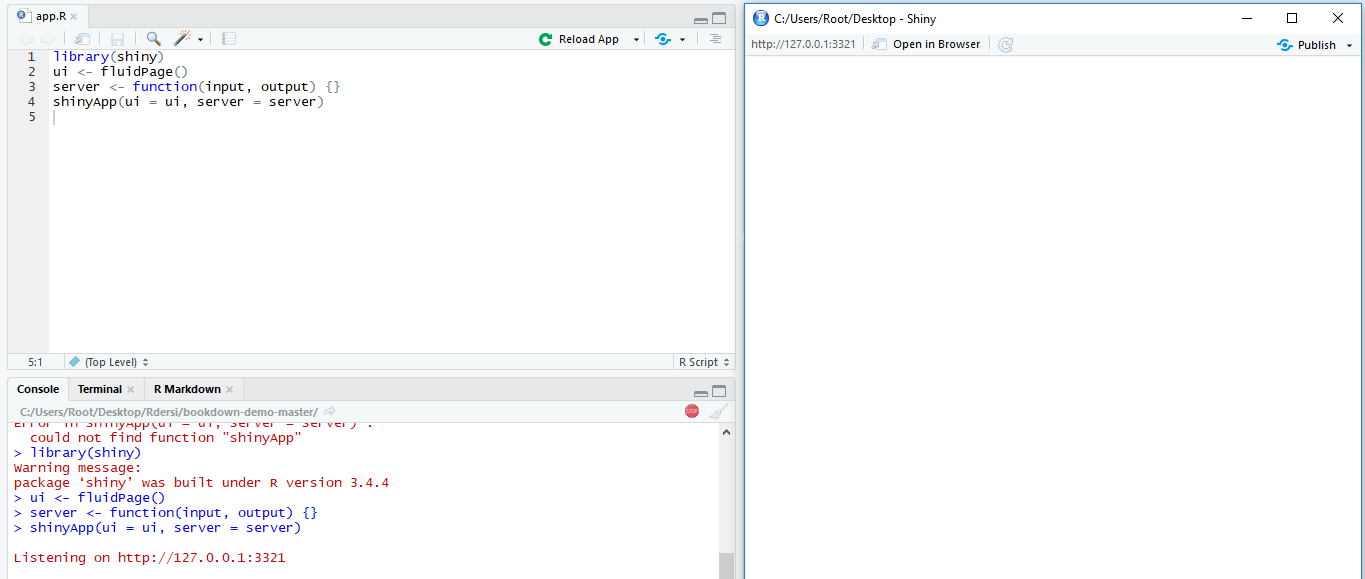
\includegraphics{resim5.png}

şeklinde bir yan pencere açılcaktır ve konsol kısmında {Listening on
\url{http://127.0.0.1:3321}} gibi bir metin yer alıyorsa uygulamanız
şuanda hiçbir problem yaşamadan çalışıyor demektir.

\section{Düzenleme}\label{duzenleme-1}

\subsection{Ui}\label{ui}

\subsubsection{Başlık}\label{baslk-1}

Uygulamaya h1() ile bir başlık ekleyebiliriz, ancak Shiny ayrıca özel
bir işlevi olan titlePanel() özelliğine de sahiptir. TitlePanel()
işlevini kullanmak, sayfanın üst kısmına görünür büyük başlık benzeri
bir metin eklemekle kalmaz, aynı zamanda web sayfasının ``resmi''
başlığını da ayarlar. Bu, tarayıcıdaki sekmenin ismine baktığınızda, bu
başlığı göreceğiniz anlamına gelir. Şimdiye kadar denediğiniz
fluidPage() 'ın üzerine yazıp, basit bir başlık ile değiştirin.

\begin{Shaded}
\begin{Highlighting}[]
\KeywordTok{fluidPage}\NormalTok{(}
  \KeywordTok{titlePanel}\NormalTok{(}\StringTok{"R Freamworkleri"}\NormalTok{)}
\NormalTok{)}
\end{Highlighting}
\end{Shaded}

\subsubsection{Sayfa Düzeni}\label{sayfa-duzeni}

Şimdiye kadar sadece metin ve HTML etiketlerini ekleyerek, her şeyin
yapılandırılmamış olduğunu ve öğelerin tek bir sütunda birbirinin altına
yığıldığını fark etmişsinizdir. Basit bir yapı eklemek için
sidebarLayout() yöntemini kullanacağız. Daha küçük bir kenar çubuğu ve
daha büyük bir ana paneli ile basit bir iki sütun düzeni sağlar.
Uygulamamızı, kullanıcının kullanabileceği tüm girişlerin kenar
çubuğunda olacak ve sonuçları sağdaki ana panelde gösterilecek şekilde
oluşturacağız.

titlePanel() kodundan sonra aşağıdaki kodu ekleyiniz.

\begin{Shaded}
\begin{Highlighting}[]
\KeywordTok{sidebarLayout}\NormalTok{(}
  \KeywordTok{sidebarPanel}\NormalTok{(}\StringTok{"Burada girdiler yer alacak"}\NormalTok{),}
  \KeywordTok{mainPanel}\NormalTok{(}\StringTok{"Çıktılar bu tarafta olacak"}\NormalTok{)}
\NormalTok{)}
\end{Highlighting}
\end{Shaded}

fluidPage() etiketi içerisindeki komutlar birbirinden virgül yardımı ile
ayrılır.

Bu ana kadar yazdığımız kodlar şöyle oluyor;

\begin{Shaded}
\begin{Highlighting}[]
\KeywordTok{library}\NormalTok{(shiny)}
\NormalTok{bcl <-}\StringTok{ }\KeywordTok{read.csv}\NormalTok{(}\StringTok{"sizin_verisetiniz.csv"}\NormalTok{, }\DataTypeTok{stringsAsFactors =} \OtherTok{FALSE}\NormalTok{)}

\NormalTok{ui <-}\StringTok{ }\KeywordTok{fluidPage}\NormalTok{(}
  \KeywordTok{titlePanel}\NormalTok{(}\StringTok{"R Freamworkleri"}\NormalTok{),}
  \KeywordTok{sidebarLayout}\NormalTok{(}
    \KeywordTok{sidebarPanel}\NormalTok{(}\StringTok{"Burada girdiler yer alacak"}\NormalTok{),}
    \KeywordTok{mainPanel}\NormalTok{(}\StringTok{"Çıktılar bu tarafta olacak"}\NormalTok{)}
\NormalTok{  )}
\NormalTok{)}

\NormalTok{server <-}\StringTok{ }\ControlFlowTok{function}\NormalTok{(input, output) \{\}}

\KeywordTok{shinyApp}\NormalTok{(}\DataTypeTok{ui =}\NormalTok{ ui, }\DataTypeTok{server =}\NormalTok{ server)}
\end{Highlighting}
\end{Shaded}

\subsubsection{Girdiler}\label{girdiler}

Girişler, kullanıcıların Shiny ile etkileşim kurmanın bir yoludur.
Shiny, kullanıcının bir uygulama ile sahip olabileceği birçok türde
etkileşimi desteklemek için birçok girdi işlevi sağlar.

textInput() kullanıcının metin girmesine izin vermek için kullanılır,
numericInput() kullanıcının bir sayı seçmesine izin verir, dateInput()
bir tarih seçmek içindir, selectInput() bir seçim kutusu (bir açılır
menü) oluşturmak içindir.

\paragraph{SliderInput()}\label{sliderinput}

Bir fiyat aralığında sayı girilmesine sağlayalım. Bunun için
sliderInput() ve numericInput() kullanabiliriz. Eğer numericInput
kullanırsak en az iki giriş kullanmamız gerekecek sınırlama için fakat
sliderInput ile bir aralık belirleyebileceğimiz için sliderInput
kullanacağız.

\begin{Shaded}
\begin{Highlighting}[]
\KeywordTok{sliderInput}\NormalTok{(}\StringTok{"fiyatGirdisi"}\NormalTok{, }\StringTok{"Fiyat"}\NormalTok{, }\DataTypeTok{min =} \DecValTok{0}\NormalTok{, }\DataTypeTok{max =} \DecValTok{100}\NormalTok{,}
            \DataTypeTok{value =} \KeywordTok{c}\NormalTok{(}\DecValTok{25}\NormalTok{, }\DecValTok{40}\NormalTok{), }\DataTypeTok{pre =} \StringTok{"₺"}\NormalTok{)}
\end{Highlighting}
\end{Shaded}

value değeri içerisinde default veriyi belirliyoruz ayrıca burada bir
fiyat aralığı olduğu için iki tane veri belirlememiz gerekiyor.

\paragraph{RadioButtons()}\label{radiobuttons}

radioButtons() için bir çeşit metin girişi istiyoruz. Ancak kullanıcının
özgürce metin girmesine izin vermek istemiyoruz çünkü kullanıcıyı sadece
birkaç seçenek ile sınırlamak istiyoruz. Amacımız için radyo düğmelerini
veya bir seçim kutusunu kullanabiliriz. Şimdi sadece birkaç seçenek
olduğundan radyo düğmeleri kullanalım, bu yüzden radioButtons()
kullanımına bakalım;

\begin{Shaded}
\begin{Highlighting}[]
\KeywordTok{radioButtons}\NormalTok{(}\StringTok{"tipGirisi"}\NormalTok{, }\StringTok{"Hangisi"}\NormalTok{,}
            \DataTypeTok{choices =} \KeywordTok{c}\NormalTok{(}\StringTok{"Tür 1"}\NormalTok{, }\StringTok{"Tür 2"}\NormalTok{, }\StringTok{"Tür 3"}\NormalTok{, }\StringTok{"Tür 4"}\NormalTok{),}
            \DataTypeTok{selected =} \StringTok{"Tür 4"}\NormalTok{)}
\end{Highlighting}
\end{Shaded}

bu kodları sidebarPanel() kodu içerisine ekliyoruz. Ayrıca virgül ile
ayrımayı unutmamız gerekiyor.

\paragraph{SelectInput()}\label{selectinput}

selectInput() varsayalım bir sehir seçtimek istiyoruz bu durumda en
uygun giriş tipi muhtemelen seçim kutusudur. SelectInput() ile bir giriş
işlevi oluşturalım. Şimdilik sadece Ankara, Istanbul, Izmir ve Bursa
gibi seçenekler sunalım;

\begin{Shaded}
\begin{Highlighting}[]
\KeywordTok{selectInput}\NormalTok{(}\StringTok{"sehirSecimi"}\NormalTok{, }\StringTok{"Sehirler"}\NormalTok{,}
            \DataTypeTok{choices =} \KeywordTok{c}\NormalTok{(}\StringTok{"Ankara"}\NormalTok{, }\StringTok{"Bursa"}\NormalTok{, }\StringTok{"Istanbul"}\NormalTok{,}\StringTok{"Izmir"}\NormalTok{))}
\end{Highlighting}
\end{Shaded}

\paragraph{Daha Fazlası}\label{daha-fazlas-1}

Yukarıdakilerden daha fazla widget ihtiyacınız olursa
\href{https://shiny.rstudio.com/tutorial/written-tutorial/lesson3/}{buradan}
ve
\href{https://shiny.rstudio.com/tutorial/written-tutorial/lesson4/}{buradaki}
ingilizce kaynaktan yararlanabilirsiniz.

\subsection{Server}\label{server}

Bu alanda daha çok düzenleme dışında ne yapacağımızla ilgileneceğiz yani
seçilen parametre sonucunda uygulmayı nası çalıştıracağımızı
inceleyeceğiz.

Öncelikle aşağıdaki koda bakalım;

\begin{Shaded}
\begin{Highlighting}[]
\NormalTok{output}\OperatorTok{$}\NormalTok{coolplot <-}\StringTok{ }\KeywordTok{renderPlot}\NormalTok{(\{}
  \KeywordTok{plot}\NormalTok{(}\KeywordTok{rnorm}\NormalTok{(}\DecValTok{100}\NormalTok{))}
\NormalTok{\})}
\end{Highlighting}
\end{Shaded}

Bu basit kod ilk iki kuralı gösterir: renderPlot() işlevinin içinde bir
çizim oluşturuyoruz ve çıktı listesindeki coolplot'a atıyoruz. Coolplot
bir plotOutput olarak tanımlandığından, renderPlot işlevini
kullanmalıyız ve renderPlot işlevinin içinde bir çizim oluşturmalıyız.
Yukarıdaki kodu sunucu işlevinin içine eklerseniz, uygulamada 100
rastgele nokta içeren bir alan görmelisiniz.

Şimdi ggplot kullanarak bir görselleştirme yapalım. Hem değerlerimiz
arasında değişiklik yaptığımızda hem de filtreleme işlemini
kullanacağımız ayrıca ggplot ile görselleştirme yapacağımız için
uygulamamızın en üstüne aşağıdaki kütüphaneleri ekleyelim;

\begin{Shaded}
\begin{Highlighting}[]
\KeywordTok{library}\NormalTok{(ggplot2)}
\KeywordTok{library}\NormalTok{(dplyr)}
\end{Highlighting}
\end{Shaded}

\textbf{Not:} Eğer hata alıyorsanız paketlerin sisteminizde kurulu olup
olmadığına bakınız.

dplyr kütüphanesini filtreleme işlemleri için aktifleştirdik. Şimdi
gelelim seçimler ile kullanıcı arayüzünde değişiklikler sağlamaya;

\begin{Shaded}
\begin{Highlighting}[]
\NormalTok{output}\OperatorTok{$}\NormalTok{coolplot <-}\StringTok{ }\KeywordTok{renderPlot}\NormalTok{(\{}
\NormalTok{  filtered <-}
\StringTok{    }\NormalTok{verisetiniz }\OperatorTok
\StringTok{    }\KeywordTok{filter}\NormalTok{(Fiyat }\OperatorTok{>=}\StringTok{ }\NormalTok{input}\OperatorTok{$}\NormalTok{fiyatGirdisi[}\DecValTok{1}\NormalTok{],}
\NormalTok{           Fiyat }\OperatorTok{<=}\StringTok{ }\NormalTok{input}\OperatorTok{$}\NormalTok{fiyatGirdisi[}\DecValTok{2}\NormalTok{],}
\NormalTok{           Hangisi }\OperatorTok{==}\StringTok{ }\NormalTok{input}\OperatorTok{$}\NormalTok{tipGirisi,}
\NormalTok{           Sehirler }\OperatorTok{==}\StringTok{ }\NormalTok{input}\OperatorTok{$}\NormalTok{sehirSecimi}
\NormalTok{    )}
  \KeywordTok{ggplot}\NormalTok{(filtered, }\KeywordTok{aes}\NormalTok{(veriseti_icindekialan)) }\OperatorTok{+}
\StringTok{    }\KeywordTok{geom_histogram}\NormalTok{()}
\NormalTok{\})}\ErrorTok{)}
\end{Highlighting}
\end{Shaded}

Yukarıdaki kod bloğu içerisinde filtered diye bir alan oluşturduk ve
seçimlerimizi bu değişkende topladık. ``verisetiniz'' yazan alan eğer
uygulamaya bir veri seti eklerseniz bu alana ekleyeceğiniz anlamına
gelir. (Verisetini burada değil kodun üst kısımlarında tanımlayıp sadece
atadığınız değişken adını yazmanız gerekir.) ggplot içerisinde ise
değişkenlerimiz ile beraber varsa verisetine ait alan ile birleştirilip
bir görsel oluşturulur. Bu kodlar ile beraber kullanıcıya interaktif bir
web uygulaması kullanması sağlanmış olur.

\subsubsection{Genel Bakış}\label{genel-baks}

\begin{Shaded}
\begin{Highlighting}[]
\KeywordTok{library}\NormalTok{(shiny)}
\KeywordTok{library}\NormalTok{(ggplot2)}
\KeywordTok{library}\NormalTok{(dplyr)}

\NormalTok{bcl <-}\StringTok{ }\KeywordTok{read.csv}\NormalTok{(}\StringTok{"bcl-data.csv"}\NormalTok{, }\DataTypeTok{stringsAsFactors =} \OtherTok{FALSE}\NormalTok{)}

\NormalTok{ui <-}\StringTok{ }\KeywordTok{fluidPage}\NormalTok{(}
  \KeywordTok{titlePanel}\NormalTok{(}\StringTok{"R Freamworkleri"}\NormalTok{),}
  \KeywordTok{sidebarLayout}\NormalTok{(}
    \KeywordTok{sidebarPanel}\NormalTok{(}
      \KeywordTok{sliderInput}\NormalTok{(}\StringTok{"fiyatGirdisi"}\NormalTok{, }\StringTok{"Fiyat"}\NormalTok{, }\DataTypeTok{min =} \DecValTok{0}\NormalTok{, }\DataTypeTok{max =} \DecValTok{100}\NormalTok{,}
            \DataTypeTok{value =} \KeywordTok{c}\NormalTok{(}\DecValTok{25}\NormalTok{, }\DecValTok{40}\NormalTok{), }\DataTypeTok{pre =} \StringTok{"₺"}\NormalTok{),}
      \KeywordTok{radioButtons}\NormalTok{(}\StringTok{"tipGirisi"}\NormalTok{, }\StringTok{"Hangisi"}\NormalTok{,}
            \DataTypeTok{choices =} \KeywordTok{c}\NormalTok{(}\StringTok{"Tür 1"}\NormalTok{, }\StringTok{"Tür 2"}\NormalTok{, }\StringTok{"Tür 3"}\NormalTok{, }\StringTok{"Tür 4"}\NormalTok{),}
            \DataTypeTok{selected =} \StringTok{"Tür 4"}\NormalTok{),}
      \KeywordTok{selectInput}\NormalTok{(}\StringTok{"sehirSecimi"}\NormalTok{, }\StringTok{"Sehirler"}\NormalTok{,}
            \DataTypeTok{choices =} \KeywordTok{c}\NormalTok{(}\StringTok{"Ankara"}\NormalTok{, }\StringTok{"Bursa"}\NormalTok{, }\StringTok{"Istanbul"}\NormalTok{,}\StringTok{"Izmir"}\NormalTok{))}
\NormalTok{    ),}
    \KeywordTok{mainPanel}\NormalTok{(}
      \KeywordTok{plotOutput}\NormalTok{(}\StringTok{"coolplot"}\NormalTok{),}
      \KeywordTok{br}\NormalTok{(), }\KeywordTok{br}\NormalTok{(),}
      \KeywordTok{tableOutput}\NormalTok{(}\StringTok{"results"}\NormalTok{)}
\NormalTok{    )}
\NormalTok{  )}
\NormalTok{)}

\NormalTok{server <-}\StringTok{ }\ControlFlowTok{function}\NormalTok{(input, output) \{}
\NormalTok{  output}\OperatorTok{$}\NormalTok{coolplot <-}\StringTok{ }\KeywordTok{renderPlot}\NormalTok{(\{}
\NormalTok{  filtered <-}
\StringTok{    }\NormalTok{verisetiniz }\OperatorTok
\StringTok{    }\KeywordTok{filter}\NormalTok{(Fiyat }\OperatorTok{>=}\StringTok{ }\NormalTok{input}\OperatorTok{$}\NormalTok{fiyatGirdisi[}\DecValTok{1}\NormalTok{],}
\NormalTok{           Fiyat }\OperatorTok{<=}\StringTok{ }\NormalTok{input}\OperatorTok{$}\NormalTok{fiyatGirdisi[}\DecValTok{2}\NormalTok{],}
\NormalTok{           Hangisi }\OperatorTok{==}\StringTok{ }\NormalTok{input}\OperatorTok{$}\NormalTok{tipGirisi,}
\NormalTok{           Sehirler }\OperatorTok{==}\StringTok{ }\NormalTok{input}\OperatorTok{$}\NormalTok{sehirSecimi}
\NormalTok{    )}
  \KeywordTok{ggplot}\NormalTok{(filtered, }\KeywordTok{aes}\NormalTok{(veriseti_icindekialan)) }\OperatorTok{+}
\StringTok{    }\KeywordTok{geom_histogram}\NormalTok{()}
\NormalTok{\}}

\KeywordTok{shinyApp}\NormalTok{(}\DataTypeTok{ui =}\NormalTok{ ui, }\DataTypeTok{server =}\NormalTok{ server)}
\end{Highlighting}
\end{Shaded}

Aşağıdaki resimde yukarıdaki kodun çalıştırılmış halini inceleyelim.

\begin{figure}
\centering
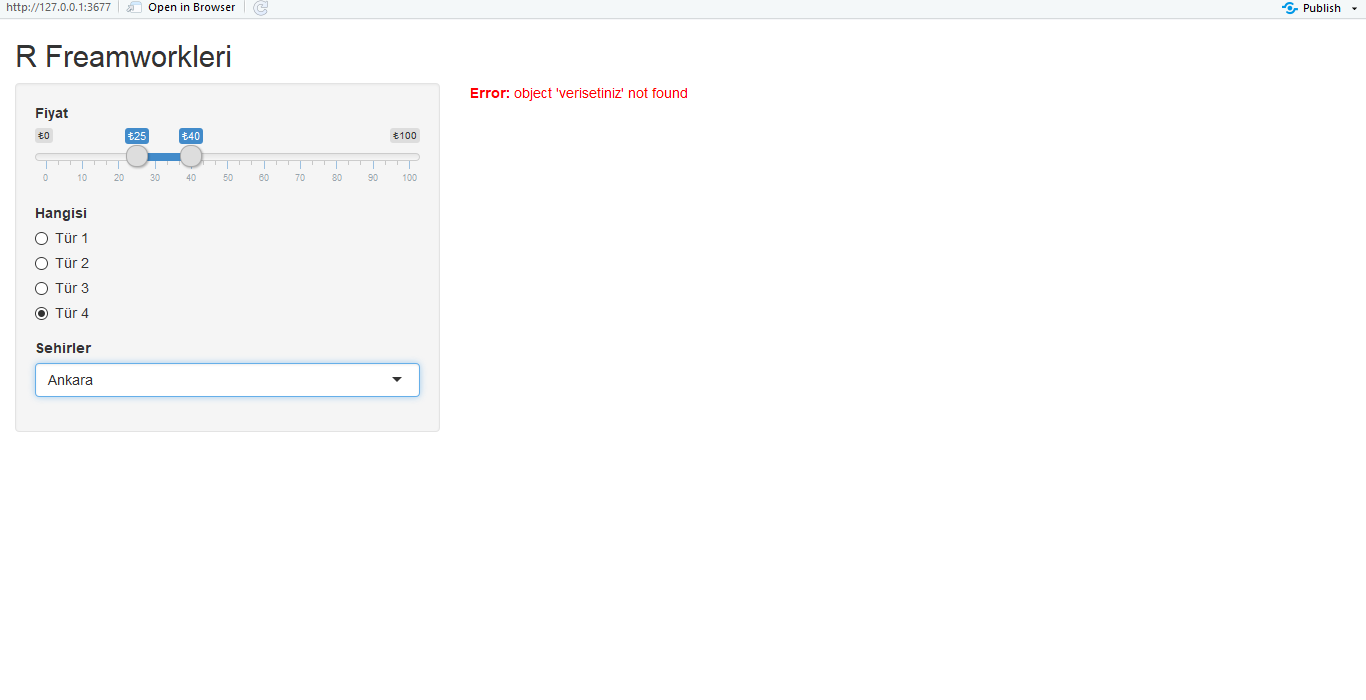
\includegraphics{resim6.png}
\caption{}
\end{figure}

Bu resimde bir veri setimiz olmadığı için uygulama hata veriyor bir veri
seti ekleyip tekrar deneyelim; 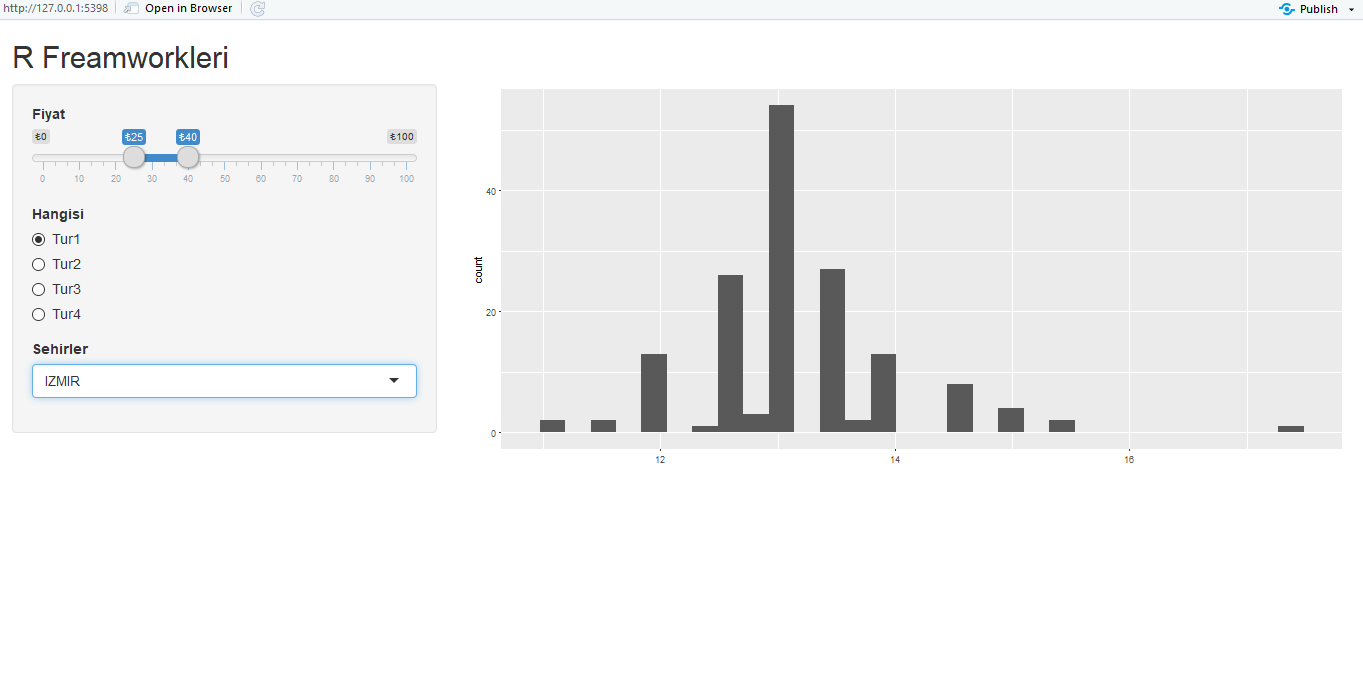
\includegraphics{resim7.png}

görüldüğü üzere uygulamamız çalışıyor.

\section{Yayınlama}\label{yaynlama}

Uygulamanızı hazırladınız ve web üzerinde yayınlamanız gerekiyor işte bu
noktada \href{http://www.shinyapps.io/}{shinyapps.io} size belli bir
sayıya kadar barındırma hizmeti sunar. RStudio entegre olan bu hizmet
size uygulamanız ile ilgili istatislikler verir.

Öncelikle Uygulamanızı shinyapps.io üzerinde barındırma uygulaması,
uygulamanızı çevrimiçi hale getirmenin kolay ve önerilen yoludur.
\href{http://www.shinyapps.io/}{shinyapps.io} adresine gidin ve yeni bir
hesap için kaydolun. Uygulamanızı yayınlamaya hazır olduğunuzda,
RStudio'daki ``Publish Application'' düğmesini tıklayın ve talimatlarını
uygulayın. İlk kez bir çift paket yüklemeniz istenebilir.
Shinyapps.io'ya başarılı bir yüklemeden sonra, uygulamanıza tarayıcıda
yönlendirileceksiniz. Bu URL'yi çevrenize göstermek için yazdığınız
harika bir uygulama olarak kullanabilirsiniz.

\begin{figure}
\centering
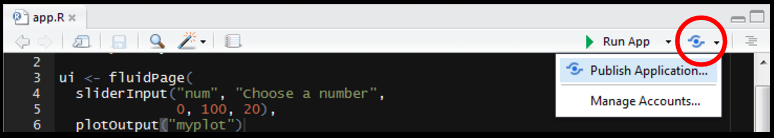
\includegraphics{resim8.png}
\caption{}
\end{figure}

\chapter{Swirl}\label{swirl}

Swirl diğerlerinden farklı olarak isterseniz R derslerini
öğrenebileceğiniz isterseniz ders olşturup insanların bu dersler
sayesinde R konularını öğrenmelerini sağlayabileceğiniz freamworktür.

\section{Gereklilikler}\label{gereklilikler-3}

RStudio'yu açıp konsol kısmına aşağıdaki komutu yapıştırarak gerekli
paketlerin kurulmasını sağlayabilirsiniz;

Dersi öğrenmek için;

\begin{Shaded}
\begin{Highlighting}[]
\KeywordTok{install.packages}\NormalTok{(}\StringTok{"swirl"}\NormalTok{)}
\end{Highlighting}
\end{Shaded}

Ders oluşturmak için;

\begin{Shaded}
\begin{Highlighting}[]
\KeywordTok{install.packages}\NormalTok{(}\KeywordTok{c}\NormalTok{(}\StringTok{"swirl"}\NormalTok{, }\StringTok{"swirlify"}\NormalTok{))}
\end{Highlighting}
\end{Shaded}

\section{Başlangıç}\label{baslangc-2}

\subsection{Dersi Öğrenmek İçin}\label{dersi-ogrenmek-icin}

Ders öğrenmek için;

\begin{Shaded}
\begin{Highlighting}[]
\KeywordTok{library}\NormalTok{(swirl)}
\end{Highlighting}
\end{Shaded}

kütüphanesini etkinleştirdikten sonra

\begin{Shaded}
\begin{Highlighting}[]
\KeywordTok{swirl}\NormalTok{()}
\end{Highlighting}
\end{Shaded}

kodunu çalıştırarak dersi aktifleştirelim ve içersindeki dersi öğrenmeye
başlayalım. 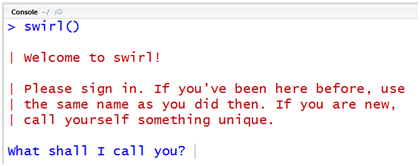
\includegraphics{resim10.png}

\subsection{Ders Oluşturmak İçin}\label{ders-olusturmak-icin}

Gerekli paketleri indirdik ve şimdi ders oluşturmamız gerekiyor. İlk
olarak ``swirlify'' kütüphanesini aktif hale getirmemiz gerekiyor.

\begin{Shaded}
\begin{Highlighting}[]
\KeywordTok{library}\NormalTok{(swirlify)}
\end{Highlighting}
\end{Shaded}

Kütüphane aktifleştirmede bir sıkıntı yoksa sırada dersimizi oluşturmaya
geldi. ``new\_lesson()'' komutu ile yeni ve ham bir ders
oluşturabiliriz.

\begin{Shaded}
\begin{Highlighting}[]
\KeywordTok{new_lesson}\NormalTok{(}\StringTok{"KursunAdi"}\NormalTok{, }\StringTok{"DersinAdi"}\NormalTok{)}
\end{Highlighting}
\end{Shaded}

şeklinde dersimizi oluşturabiliriz. Bu komutu aktifleştirdikten sonra
aşağıdaki gibi bir dosya sistemine sahip olacağız.

\begin{Shaded}
\begin{Highlighting}[]
\NormalTok{─ DersinAdi}
\NormalTok{  └─ KursunAdi}
\NormalTok{     ├─ lesson.yaml}
\NormalTok{     ├─ initLesson.R}
\NormalTok{     ├─ dependson.txt}
\NormalTok{     └─ customTests.R}
\end{Highlighting}
\end{Shaded}

Peki bu dosyalar içerisinde neler yer alıyor.\\
\textbf{lesson.yaml:} Soruların yazıldığı alan burasıdır. Sorular
yazılır eğer tanımlı ise bir fonksiyona yönlendirilir veya kendi
içerisinde basit bir şekilde değerlendirilir.\\
\textbf{initLesson.R:} Genellikle veri yüklemek veya çevresel
değişkenler oluşturmak için kullanılan ders başlamadan önce çalışan bir
R betiğidir.\\
\textbf{depenson.txt:} Bir veriyi tanıtmak için kullanılan R
betiğidir.\\
\textbf{customTests.R:} Öğrencilerin cevapları için kendi testlerinizi
yazabileceğiniz yerdir.

\section{Düzenleme}\label{duzenleme-2}

\subsection{Dersi Öğrenmek İçin}\label{dersi-ogrenmek-icin-1}

Gelen paket içerisindeki dersler yetersiz geldiğinde aşağıdaki kodu
kullanark yeni ders ekleyebilirsiniz.

\begin{Shaded}
\begin{Highlighting}[]
\KeywordTok{library}\NormalTok{(swirl)}
\KeywordTok{install_course}\NormalTok{(}\StringTok{"Kurs_adi"}\NormalTok{)}
\KeywordTok{swirl}\NormalTok{()}
\end{Highlighting}
\end{Shaded}

Eğer dersi indirdiyseniz;

\begin{Shaded}
\begin{Highlighting}[]
\KeywordTok{library}\NormalTok{(swirl)}
\KeywordTok{install_course_zip}\NormalTok{(}\StringTok{"path/to/file/here/dosya_adi.zip"}\NormalTok{, }\DataTypeTok{multi=}\OtherTok{TRUE}\NormalTok{, }
                   \DataTypeTok{which_course=}\StringTok{"Kurs_adi"}\NormalTok{)}
\KeywordTok{swirl}\NormalTok{()}
\end{Highlighting}
\end{Shaded}

ve dersi kaldırmak için;

\begin{Shaded}
\begin{Highlighting}[]
\KeywordTok{uninstall_course}\NormalTok{(}\StringTok{"Kurs_adi"}\NormalTok{)}
\end{Highlighting}
\end{Shaded}

\subsection{Dersi Oluşturmak İçin}\label{dersi-olusturmak-icin}

\subsubsection{Lesson.yaml}\label{lesson.yaml}

Yukarıda bahsedildiği gibi soruların ve cevapların yer aldığı bölüm
aşağıdaki şekilde düzenlenir.

\begin{Shaded}
\begin{Highlighting}[]
\OperatorTok{-}\StringTok{ }\NormalTok{Class}\OperatorTok{:}\StringTok{ }\NormalTok{cmd_question}
\NormalTok{  Output}\OperatorTok{:}\StringTok{ }\NormalTok{R konsolu içerisinde }\DecValTok{2}\NormalTok{ ve }\DecValTok{2}\NormalTok{ sayılarını toplayınız.}
\NormalTok{  CorrectAnswer}\OperatorTok{:}\StringTok{ }\DecValTok{2} \OperatorTok{+}\StringTok{ }\DecValTok{2}
\NormalTok{  AnswerTests}\OperatorTok{:}\StringTok{ }\KeywordTok{omnitest}\NormalTok{(}\DataTypeTok{correctExpr=}\StringTok{'2 + 2'}\NormalTok{)}
\NormalTok{  Hint}\OperatorTok{:}\StringTok{ }\NormalTok{Just type }\DecValTok{2} \OperatorTok{+}\StringTok{ }\DecValTok{2}\NormalTok{.}
\end{Highlighting}
\end{Shaded}

\subsubsection{depenson.txt}\label{depenson.txt}

Bu alanda düz metin olarak fonksiyonlar hakkında bilgi verebilirsiniz.

\begin{Shaded}
\begin{Highlighting}[]
\NormalTok{Bu fonksiyon ..... işlemlerini gerçekleştirmektedir.}
\end{Highlighting}
\end{Shaded}

\subsubsection{initLesson.R}\label{initlesson.r}

Bir R betiğinde olduğu gibi değişkenlerinizi ve verilerinizi ekledeğiniz
bölümün örneği aşağıdaki gibidir;

\begin{Shaded}
\begin{Highlighting}[]
\KeywordTok{library}\NormalTok{(dplyr)}

\CommentTok{# Sayı aralığı}
\NormalTok{.ng <-}\StringTok{ }\DecValTok{5}
\CommentTok{#Öğrenciler/Gruplar için maksimum değer}
\NormalTok{.gmax <-}\StringTok{ }\DecValTok{8}

\CommentTok{# Kolon başlıkları değerlerdir, değer isimleri değil}

\KeywordTok{set.seed}\NormalTok{(}\DecValTok{1234}\NormalTok{)}
\NormalTok{students <-}\StringTok{ }\KeywordTok{data.frame}\NormalTok{(}
  \DataTypeTok{grade =}\NormalTok{ LETTERS[}\DecValTok{1}\OperatorTok{:}\NormalTok{.ng],}
  \DataTypeTok{male =} \KeywordTok{sample}\NormalTok{(}\DecValTok{0}\OperatorTok{:}\NormalTok{.gmax, .ng, }\DataTypeTok{replace =} \OtherTok{TRUE}\NormalTok{),}
  \DataTypeTok{female =} \KeywordTok{sample}\NormalTok{(}\DecValTok{0}\OperatorTok{:}\NormalTok{.gmax, .ng, }\DataTypeTok{replace =} \OtherTok{TRUE}\NormalTok{)}
\NormalTok{)}
\end{Highlighting}
\end{Shaded}

\subsubsection{customTests.R}\label{customtests.r}

Kendi fonksiyonalrınızı oluşturacağınız bu bölümde topladığınız verileri
işlemler ile beraber çalıştırarak aldığınız sonuçları kullanıcıya
döndüreceğiniz dosyadır. Örne olarak;

\begin{Shaded}
\begin{Highlighting}[]
\CommentTok{# Bir kullanıcının komuta göre doğrudan girdiği veya hesaplandığı veriyi alın}
\NormalTok{getVal <-}\StringTok{ }\ControlFlowTok{function}\NormalTok{()\{}
  \KeywordTok{getState}\NormalTok{()}\OperatorTok{$}\NormalTok{val}
\NormalTok{\}}
\end{Highlighting}
\end{Shaded}

\section{Yayınlama}\label{yaynlama-1}

Kendi dersinizi oluşturdunuz ve artık bunu öğrenmek isteyenlere sunmak
istiyorsunuz o halde dersi bir dosya halinde nasıl çıktı alacağımıza bir
bakalım;

\begin{Shaded}
\begin{Highlighting}[]
\KeywordTok{set_lesson}\NormalTok{()}
\end{Highlighting}
\end{Shaded}

bu komut ile dersinizi ayarlamanız gerekiyor daha sonra

\begin{Shaded}
\begin{Highlighting}[]
\KeywordTok{pack_course}\NormalTok{()}
\end{Highlighting}
\end{Shaded}

komutu ile \textbf{.swc} uzantılı bir dosya oluşturduk. Bu dosyayı
normal bir dosya gibi paylaşabilirsiniz ve ihtiyacınız olduğunda
\textbf{install\_course()} komutu ile dersi çalıştırabilirsiniz.

\chapter{RWebsite}\label{rwebsite}

R ile yapılan bir sürü uygulama arasında web sitesi yapımıda bunların
arasında yerini almış olanlardan birisdir. Bu sayede kişisel, proje,
paket ve blog sitenizi oluşturabilirsiniz.

\section{Gereklilikler}\label{gereklilikler-4}

Websitesi ve Blog sayfaları hazırlamanız için aşağıdaki paketlere
ihtiyacınız vardır.

\begin{Shaded}
\begin{Highlighting}[]
\KeywordTok{install.packages}\NormalTok{(}\StringTok{"rmarkdown"}\NormalTok{)}
\KeywordTok{install.packages}\NormalTok{(}\StringTok{"blogdown"}\NormalTok{)}
\NormalTok{blogdown}\OperatorTok{::}\KeywordTok{install_hugo}\NormalTok{()}
\end{Highlighting}
\end{Shaded}

\section{Başlangıç}\label{baslangc-3}

Blog ve websitesi için giriş aşamasında neler yapılması gerektiğini
inceleyeceğiz.

\subsection{Website}\label{website}

Başlangıç olarak iki sayfadan oluşan basit bir site oluşturalım. İlk
olarak bir ayar dosyası oluşturmamız gerekiyor. Bu dosyanın adı
**/\_site.yml** olmalıdır. Bu dosya içerisinde sayfaların yolları ve
site adı gibi bazı bilgiler yer alacaktır.

**\_site.yml**

\begin{Shaded}
\begin{Highlighting}[]
\NormalTok{name: "r-freamworkleri"}
\NormalTok{navbar:}
\NormalTok{  title: "R Freamworkleri"}
\NormalTok{  left:}
\BaseNTok{    - text: "Ana Sayfa"}
\BaseNTok{      href: index.html}
\BaseNTok{    - text: "Hakkında"}
\BaseNTok{      href: about.html}
\end{Highlighting}
\end{Shaded}

\textbf{index.Rmd}

\begin{Shaded}
\begin{Highlighting}[]
\NormalTok{---}
\NormalTok{title: "My Website"}
\NormalTok{---}

\NormalTok{Hello, Website!}
\end{Highlighting}
\end{Shaded}

\textbf{about.Rmd}

\begin{Shaded}
\begin{Highlighting}[]
\NormalTok{---}
\NormalTok{title: "About This Website"}
\NormalTok{---}

\NormalTok{More about this website.}
\end{Highlighting}
\end{Shaded}

benzeri bir yapıya sahip olmaları gerekiyor.

\subsection{Blog}\label{blog}

Başlangıç olarak basit bir blog sitesi oluşturalım.

\begin{Shaded}
\begin{Highlighting}[]
\NormalTok{blogdown::new_site()}
\end{Highlighting}
\end{Shaded}

bu komut ile örnek template ile yeni bir blog sayfası oluşturulur. İlk
olarak bu oluşan sayfanın bir canlı önizlemesini alalım.

\begin{Shaded}
\begin{Highlighting}[]
\NormalTok{blogdown::serve_site()}
\end{Highlighting}
\end{Shaded}

Şimdi oluşturduğumuz sitenin alt dosyalarını inceleyelim.
\textbf{config.toml} Bu dosya içerisinde temel ayarları belirleyeceğiz.
Site başlığı, dili, teması, diğer sayfalar ile olan bağlantısı gibi.
config.toml dosyası aşağıdaki gibi olmalıdır.

\begin{Shaded}
\begin{Highlighting}[]
\NormalTok{baseurl = "/"}
\NormalTok{languageCode = "en-us"}
\NormalTok{title = "A Hugo website"}
\NormalTok{theme = "hugo-lithium"}

\NormalTok{[[menu.main]]}
\BaseNTok{    name = "About"}
\BaseNTok{    url = "/about/"}
\NormalTok{[[menu.main]]}
\BaseNTok{    name = "GitHub"}
\BaseNTok{    url = "https://github.com/rstudio/blogdown"}
\NormalTok{[[menu.main]]}
\BaseNTok{    name = "Twitter"}
\BaseNTok{    url = "https://twitter.com/rstudio"}
\end{Highlighting}
\end{Shaded}

Blog sayfanız için yeni temalara
\href{http://themes.gohugo.io/}{buradan} ulaşabilirsiniz. Yeni temanızı
aşağıdaki şekilde kurabilirsiniz.

\begin{Shaded}
\begin{Highlighting}[]
\NormalTok{blogdown}\OperatorTok{::}\KeywordTok{new_site}\NormalTok{(}\DataTypeTok{theme =} \StringTok{"gcushen/hugo-academic"}\NormalTok{)}
\end{Highlighting}
\end{Shaded}

\section{Düzenleme}\label{duzenleme-3}

\subsection{Website}\label{website-1}

Bir web sitesi içerisinde eklemeniz gereken çeşitli öğeler(Css,
üstbilgi, altbilgi) vardır.

**\_site.yml**

\begin{Shaded}
\begin{Highlighting}[]
\NormalTok{name: "r-freamworkleri"}
\NormalTok{navbar:}
\NormalTok{  title: "R Freamworkleri"}
\NormalTok{  left:}
\BaseNTok{    - text: "Ana Sayfa"}
\BaseNTok{      href: index.html}
\BaseNTok{    - text: "Hakkında"}
\BaseNTok{      href: about.html}
\NormalTok{output:}
\NormalTok{  html_document:}
\BaseNTok{    theme: cosmo}
\BaseNTok{    highlight: textmate}
\BaseNTok{    include:}
\BaseNTok{      after_body: footer.html}
\BaseNTok{    css: styles.css}
\end{Highlighting}
\end{Shaded}

\textbf{footer.html}

\begin{Shaded}
\begin{Highlighting}[]
\KeywordTok{<p>}\NormalTok{Copyright }\DecValTok{&copy;}\NormalTok{ 2018 RFreamworkleri. Tüm Hakları Saklıdır.}\KeywordTok{</p>}
\end{Highlighting}
\end{Shaded}

\textbf{style.css}

\begin{Shaded}
\begin{Highlighting}[]
\NormalTok{blockquote }\KeywordTok{\{}
  \KeywordTok{font-style:} \DataTypeTok{italic}
\KeywordTok{\}}
\end{Highlighting}
\end{Shaded}

render sırasında ortak öğeler ile sayfaların tek tek birleştirilerek
istenilen şekilde bir site oluşturulmasını sağlamaktadır.

\subsection{Blog}\label{blog-1}

\subsubsection{Yeni Post}\label{yeni-post}

Her blog sitesinde olduğu gibi düzenli post atmanız gerektiği için
yeniden sayfalarla uğraşmak yerine aşağıdaki komutu kullanarak tema
dosyanıza uygun olarak yeni bir post sayfası oluşturabilirsiniz.

\begin{Shaded}
\begin{Highlighting}[]
\NormalTok{blogdown}\OperatorTok{::}\KeywordTok{new_post}\NormalTok{()}
\end{Highlighting}
\end{Shaded}

\subsubsection{Sayfa Düzenlemeleri}\label{sayfa-duzenlemeleri}

Sayfa düzenlemeleri web sitesinin yapımı ile benzerlik göstermektedir.

\section{Çıktı}\label{ckt}

\subsection{Website}\label{website-2}

Her önizleme aldığınızda siteniz \_site içerisinde hazır hale gelir. Bu
aşamadan sonra yapmanız gereken çıktıları alıp sunucunuza eklemek
olacaktır.

\subsection{Blog}\label{blog-2}

Blog yayınlamada ise birkaç alanda depolanabileceği için çeşitlilikler
göstermektedir. Ücretsiz ve stabil olmasından dolayı github üzerinden
yayınlama işlemlerine göz atalım. Bu noktada,
\textless{}username.github.io\textgreater{} deponuza sahip olduğunuz
veya yeni oluşturduğunuz ya da yerel makinenize klonladınız. Ayrıca,
Hugo'yu sitenizin config.toml dosyasındaki publishDir =
``\textless{}username.github.io'' seçeneğini kullanarak sitenizi aynı
depoya yayınlamasını istediniz. Sadece birkaç adım kaldı!

\begin{verbatim}
Hugo’yu sitenize build_site () ile (argümanlar gerekmez) yapmasını söyleyin. Hugo sitenizi oluşturmayı tamamladıktan sonra, <username> .gihub.io dizininize bir göz atın, şimdi kaynak içerik deponuzun public / dizini ile aynı dosyaları içermelidir.

Terminali açın, <kullaniciadi.github.io repo> 'yı kullanarak <username> .gihub.io dizinine gidin. Tüm değiştirilen dosyaları hazırlayın, değişikliklerinizi yapın ve yeni sitenizi GitHub'a aktarın.
\end{verbatim}

Bu kadar! \url{https://kullanıcıadı.github.io} adresindeki yeni web
sitenize gidin ve neler yaptığınıza bir bakın!

\bibliography{book.bib,packages.bib}


\end{document}
